%%%%%%%%%%%%%%%%%%%%%%%%%%%%%%%%%%%%%%%%%%%%%%%%%%%%%%%%%%
%%%%%%%%%%%%%%%%%%%%%%%%%%%%%%%%%%%%%%%%%%%%%%%%%%%%%%%%%%
\subsection{Overview}
%%%%%%%%%%%%%%%%%%%%%%%%%%%%%%%%%%%%%%%%%%%%%%%%%%%%%%%%%%
%%%%%%%%%%%%%%%%%%%%%%%%%%%%%%%%%%%%%%%%%%%%%%%%%%%%%%%%%%

%%%%%%%%%%%%%%%%%%%%%%%%%%%%%%%%%%%%%%%%%%%%%%%%%%%%%%%%%%
\frame {\frametitle{Disclaimer}
%%%%%%%%%%%%%%%%%%%%%%%%%%%%%%%%%%%%%%%%%%%%%%%%%%%%%%%%%%
  \begin{itemize}
  \item \textbf{MapReduce APIs}
    \begin{itemize}
    \item Fast evolving
    \item Sometimes confusing
    \end{itemize}

\vspace{40pt} 

  \item \textbf{Do {\color{red}NOT} rely on this slide deck as a reference}
    \begin{itemize}
      \item Use appropriate API docs
      \item Use Eclipse
    \end{itemize}
  \end{itemize}
}

%%%%%%%%%%%%%%%%%%%%%%%%%%%%%%%%%%%%%%%%%%%%%%%%%%%%%%%%%%
\frame {\frametitle{Anatomy of a MapReduce Job Run}
%%%%%%%%%%%%%%%%%%%%%%%%%%%%%%%%%%%%%%%%%%%%%%%%%%%%%%%%%%
   \begin{center}
      \framebox{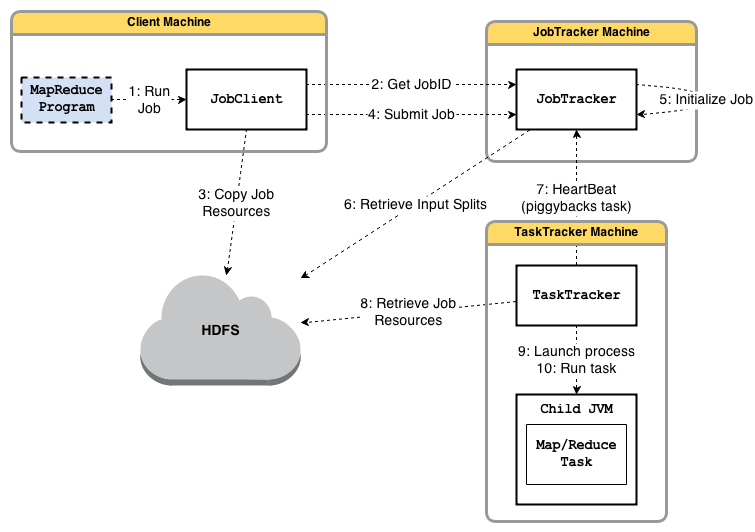
\includegraphics[scale=0.36]{./Figures/mapreduce}}      
    \end{center}
}

%%%%%%%%%%%%%%%%%%%%%%%%%%%%%%%%%%%%%%%%%%%%%%%%%%%%%%%%%%
\frame {\frametitle{Job Submission}
%%%%%%%%%%%%%%%%%%%%%%%%%%%%%%%%%%%%%%%%%%%%%%%%%%%%%%%%%%
  \begin{itemize}
  \item \textbf{\texttt{JobClient} class}
    \begin{itemize}
    \item The \texttt{runJob()} method creates a new instance of a
      \textbf{JobClient}
    \item Then it calls the \texttt{submitJob()} on this class
    \end{itemize}

\vspace{20pt} 

  \item \textbf{Simple verifications on the Job}
    \begin{itemize}
    \item Is there an output directory?
    \item Are there any input splits?
    \item Can I copy the JAR of the job to HDFS?
    \end{itemize}

\vspace{20pt}

  \item \textbf{NOTE: the JAR of the job is replicated 10 times}
  \end{itemize}
}

%%%%%%%%%%%%%%%%%%%%%%%%%%%%%%%%%%%%%%%%%%%%%%%%%%%%%%%%%%
\frame {\frametitle{Job Initialization}
%%%%%%%%%%%%%%%%%%%%%%%%%%%%%%%%%%%%%%%%%%%%%%%%%%%%%%%%%%
  \begin{itemize}
  \item \textbf{The \texttt{JobTracker} is responsible for:}
    \begin{itemize}
    \item Create an object for the job
    \item Encapsulate its tasks
    \item {\color{red}Bookkeeping} with the tasks' status and progress
    \end{itemize}

    \vspace{20pt}

  \item \textbf{This is where the scheduling happens}
    \begin{itemize}
    \item \texttt{JobTracker} performs scheduling by maintaining a
      queue
    \item Queuing disciplines are pluggable
    \end{itemize}

    \vspace{20pt}

  \item \textbf{Compute mappers and reducers}
    \begin{itemize}
    \item \texttt{JobTracker} retrieves input splits (computed by
      \texttt{JobClient})
    \item Determines the number of Mappers based on the number of
      input splits
    \item Reads the configuration file to set the number of Reducers
    \end{itemize}

  \end{itemize}
}

%%%%%%%%%%%%%%%%%%%%%%%%%%%%%%%%%%%%%%%%%%%%%%%%%%%%%%%%%%
%%%%%%%%%%%%%%%%%%%%%%%%%%%%%%%%%%%%%%%%%%%%%%%%%%%%%%%%%%
\subsection{Scheduling}
%%%%%%%%%%%%%%%%%%%%%%%%%%%%%%%%%%%%%%%%%%%%%%%%%%%%%%%%%%
%%%%%%%%%%%%%%%%%%%%%%%%%%%%%%%%%%%%%%%%%%%%%%%%%%%%%%%%%%
\begin{frame}
 \begin{colorblock}{blue}{lightblue}{ }
  \begin{center}
    \textbf{Scheduling}
  \end{center}
  \end{colorblock}
\end{frame}

%%%%%%%%%%%%%%%%%%%%%%%%%%%%%%%%%%%%%%%%%%%%%%%%%%%%%%%%%%
\frame {\frametitle{Task Assignment}
%%%%%%%%%%%%%%%%%%%%%%%%%%%%%%%%%%%%%%%%%%%%%%%%%%%%%%%%%%
  \begin{itemize}
  \item\textbf{Heartbeat-based mechanism}
    \begin{itemize}
    \item \texttt{TaskTrackers} periodically send heartbeats to the
      \texttt{JobTracker}
    \item \texttt{TaskTracker} is alive
    \item Heartbeat contains also information on availability of the
      \texttt{TaskTrackers} to execute a task
    \item \texttt{JobTracker} piggybacks a task if
      \texttt{TaskTracker} is available
    \end{itemize}

    \vspace{20pt}

  \item \textbf{Selecting a task}
    \begin{itemize}
    \item \texttt{JobTracker} first needs to select a job
      (\textit{i.e.} Job scheduling)
    \item \texttt{TaskTrackers} have a fixed number of slots for map
      and reduce tasks
    \item \texttt{JobTracker} gives priority to map tasks ({\color{red}WHY?})
    \end{itemize}

    \vspace{20pt}

  \item \textbf{Data locality}
    \begin{itemize}
    \item \texttt{JobTracker} is topology aware
      \begin{itemize}
      \item Useful for map tasks
      \item Unused for reduce tasks ({\color{red}WHY?})
      \end{itemize}
    \end{itemize}

  \end{itemize} 
}

%%%%%%%%%%%%%%%%%%%%%%%%%%%%%%%%%%%%%%%%%%%%%%%%%%%%%%%%%%
\frame {\frametitle{Task Execution}
%%%%%%%%%%%%%%%%%%%%%%%%%%%%%%%%%%%%%%%%%%%%%%%%%%%%%%%%%%
  \begin{itemize}
  \item \textbf{Task Assignment is done, now \texttt{TaskTrackers} can
    execute}
    \begin{itemize}
    \item Copy the JAR from HDFS
    \item Create a local working directory
    \item Create an instance of \texttt{TaskRunner}
    \end{itemize}

    \vspace{20pt}

  \item \textbf{\texttt{TaskRunner} launches a {\color{red}child} JVM}
    \begin{itemize}
    \item This prevents bugs from stalling the \texttt{TaskTracker}
    \item A new child JVM is created per \texttt{InputSplit}
      \begin{itemize}
      \item Can be overridden by specifying JVM Reuse option, which is
        very useful for {\color{red}custom, in-memory, combiners}
      \end{itemize}
    \end{itemize}

    \vspace{20pt}

  \item \textbf{Streaming and Pipes}
    \begin{itemize}
    \item User-defined map and reduce methods need not to be in Java
    \item Streaming and Pipes allow C++ or python mappers and reducers
    \item NOTE: this feature is heavily used in industry, with some tricky downsides
    \end{itemize}
  \end{itemize}
}

%%%%%%%%%%%%%%%%%%%%%%%%%%%%%%%%%%%%%%%%%%%%%%%%%%%%%%%%%%
\frame {\frametitle{Scheduling in detail}
%%%%%%%%%%%%%%%%%%%%%%%%%%%%%%%%%%%%%%%%%%%%%%%%%%%%%%%%%%
  \begin{itemize}
  \item \textbf{FIFO Scheduler (default in vanilla Hadoop)}
    \begin{itemize}
    \item First-come-first-served
      \begin{itemize}
      \item Long jobs monopolize the cluster
      \end{itemize}
    \end{itemize}

    \vspace{20pt}

  \item \textbf{Fair Scheduler (default in Cloudera)}
    \begin{itemize}
    \item Every user gets a fair share of the cluster capacity over time
    \item Jobs are placed into pools, one for each user
      \begin{itemize}
      \item Users that submit more jobs have no more resources than oterhs
      \item Can guarantee minimum capacity per pool
      \end{itemize}
    \end{itemize}

    \vspace{20pt}

  \item \textbf{Capacity Scheduler (heavily used in Yahoo)}
    \begin{itemize}
    \item Hierarchical queues (mimic an organization)
    \item FIFO scheduling in each queue
    \item Supports priority
    \end{itemize}
  \end{itemize}
}

%%%%%%%%%%%%%%%%%%%%%%%%%%%%%%%%%%%%%%%%%%%%%%%%%%%%%%%%%%
%%%%%%%%%%%%%%%%%%%%%%%%%%%%%%%%%%%%%%%%%%%%%%%%%%%%%%%%%%
\subsection{Failures}
%%%%%%%%%%%%%%%%%%%%%%%%%%%%%%%%%%%%%%%%%%%%%%%%%%%%%%%%%%
%%%%%%%%%%%%%%%%%%%%%%%%%%%%%%%%%%%%%%%%%%%%%%%%%%%%%%%%%%
\begin{frame}
 \begin{colorblock}{blue}{lightblue}{ }
  \begin{center}
    \textbf{Failures}
  \end{center}
  \end{colorblock}
\end{frame}

%%%%%%%%%%%%%%%%%%%%%%%%%%%%%%%%%%%%%%%%%%%%%%%%%%%%%%%%%%
\frame {\frametitle{Handling Failures}
%%%%%%%%%%%%%%%%%%%%%%%%%%%%%%%%%%%%%%%%%%%%%%%%%%%%%%%%%%
  \begin{beamerboxesrounded}[shadow=true]{}
    In the real world, code is buggy, processes crash and machines fail
  \end{beamerboxesrounded}

  \begin{itemize}
  \item \textbf{Task Failure}
    \begin{itemize}
    \item Case 1: map or reduce task throws a runtime exception
      \begin{itemize}
      \item The child JVM reports back to the parent
        \texttt{TaskTracker}
      \item \texttt{TaskTracker} logs the error and marks the
        TaskAttempt as failed
      \item \texttt{TaskTracker} frees up a slot to run another task
      \end{itemize}
    \item Case 2: Hanging tasks
      \begin{itemize}
      \item \texttt{TaskTracker} notices no progress updates (timeout
        = 10 minutes)
      \item \texttt{TaskTracker} kills the child JVM\footnote{With
          streaming, you need to take care of the orphaned process.}
      \end{itemize}
      \end{itemize}
    \item \texttt{JobTracker} is notified of a failed task
      \begin{itemize}
      \item Avoids rescheduling the task on the same
        \texttt{TaskTracker}
      \item If a task fails 4 times, it is not
        re-scheduled\footnote{Exception is made for speculative execution}
      \item {\color{red}Default behavior}: if any task fails 4 times,
        the job fails
      \end{itemize}
   \end{itemize}
}

%%%%%%%%%%%%%%%%%%%%%%%%%%%%%%%%%%%%%%%%%%%%%%%%%%%%%%%%%%
\frame {\frametitle{Handling Failures}
%%%%%%%%%%%%%%%%%%%%%%%%%%%%%%%%%%%%%%%%%%%%%%%%%%%%%%%%%%
  \begin{itemize}
  \item \textbf{\texttt{TaskTracker} Failure}
    \begin{itemize}
    \item Types: crash, running very slowly
    \item Heartbeats will not be sent to \texttt{JobTracker}
    \item \texttt{JobTracker} waits for a timeout (10 minutes), then
      it removes the \texttt{TaskTracker} from its scheduling pool
    \item \texttt{JobTracker} needs to reschedule even
      \textit{completed} tasks ({\color{red}WHY?})
    \item \texttt{JobTracker} needs to reschedule tasks in progress
    \item \texttt{JobTracker} may even blacklist a
      \texttt{TaskTracker} if too many tasks failed
    \end{itemize}

    \vspace{20pt}

  \item \textbf{\texttt{JobTracker} Failure}
    \begin{itemize}
    \item Currently, Hadoop has no mechanism for this kind of failure
    \item In future (and commercial) releases:
      \begin{itemize}
      \item Multiple \texttt{JobTrackers}
      \item Use ZooKeeper as a coordination mechanisms
      \item[$\to$] {\color{red}High Availability}
      \end{itemize}
    \end{itemize}

  \end{itemize}
}

%%%%%%%%%%%%%%%%%%%%%%%%%%%%%%%%%%%%%%%%%%%%%%%%%%%%%%%%%%
%%%%%%%%%%%%%%%%%%%%%%%%%%%%%%%%%%%%%%%%%%%%%%%%%%%%%%%%%%
\subsection{Internals}
%%%%%%%%%%%%%%%%%%%%%%%%%%%%%%%%%%%%%%%%%%%%%%%%%%%%%%%%%%
%%%%%%%%%%%%%%%%%%%%%%%%%%%%%%%%%%%%%%%%%%%%%%%%%%%%%%%%%%
\begin{frame}
 \begin{colorblock}{blue}{lightblue}{ }
  \begin{center}
    \textbf{Internals}
  \end{center}
  \end{colorblock}
\end{frame}

%%%%%%%%%%%%%%%%%%%%%%%%%%%%%%%%%%%%%%%%%%%%%%%%%%%%%%%%%%
\frame {\frametitle{Shuffle and Sort}
%%%%%%%%%%%%%%%%%%%%%%%%%%%%%%%%%%%%%%%%%%%%%%%%%%%%%%%%%%
  \begin{itemize}
  \item \textbf{The MapReduce framework guarantees the input to every reducer
      to be sorted by key}
    \begin{itemize}
    \item The process by which the system sorts and transfers map
      outputs to reducers is known as {\color{red}shuffle}
    \end{itemize}

    \vspace{20pt}

  \item \textbf{Shuffle is the most important part of the framework, where the
    ``magic'' happens}
    \begin{itemize}
    \item Good understanding allows optimizing both the framework and
      the execution time of MapReduce jobs
    \end{itemize}

    \vspace{20pt}

  \item \textbf{Subject to continuous refinements}

  \end{itemize}
}

%%%%%%%%%%%%%%%%%%%%%%%%%%%%%%%%%%%%%%%%%%%%%%%%%%%%%%%%%%
\frame {\frametitle{Shuffle and Sort: Map Side}
%%%%%%%%%%%%%%%%%%%%%%%%%%%%%%%%%%%%%%%%%%%%%%%%%%%%%%%%%%
   \begin{center}
      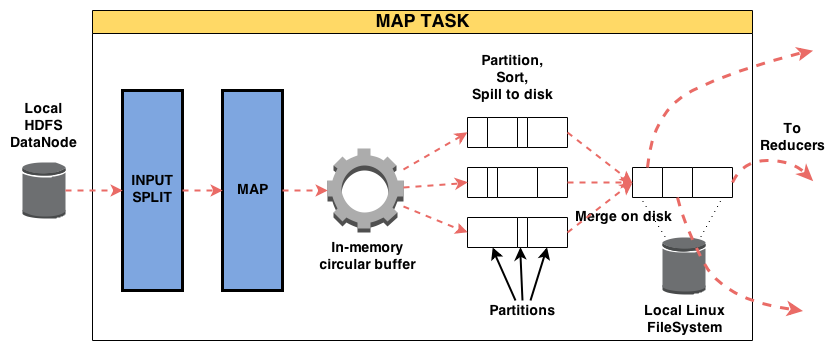
\includegraphics[scale=0.4]{./Figures/map_task}
    \end{center}
}

%%%%%%%%%%%%%%%%%%%%%%%%%%%%%%%%%%%%%%%%%%%%%%%%%%%%%%%%%%
\frame {\frametitle{Shuffle and Sort: the Map Side}
%%%%%%%%%%%%%%%%%%%%%%%%%%%%%%%%%%%%%%%%%%%%%%%%%%%%%%%%%%
  \begin{itemize}
  \item \textbf{The output of a map task is not simply written to disk}
    \begin{itemize}
    \item In memory buffering
    \item Pre-sorting
    \end{itemize}

    \vspace{20pt}
    
  \item \textbf{Circular memory buffer}
    \begin{itemize}
    \item 100 MB by default
    \item Threshold based mechanism to {\color{red}spill} buffer content to disk
    \item Map output written to the buffer {\color{red}while} spilling to disk
    \item If buffer fills up while spilling, the map task is \textbf{blocked}
    \end{itemize}
 
    \vspace{20pt}
    
  \item \textbf{Disk spills}
    \begin{itemize}
    \item Written in round-robin to a local dir
    \item Output data is partitioned corresponding to the reducers they will be sent to
    \item Within each partition, data is sorted ({\color{red}in-memory})
    \item Optionally, if there is a combiner, it is executed just after the sort phase ({\color{red}WHY?})
    \end{itemize}
  \end{itemize}
}

%%%%%%%%%%%%%%%%%%%%%%%%%%%%%%%%%%%%%%%%%%%%%%%%%%%%%%%%%%
\frame {\frametitle{Shuffle and Sort: the Map Side}
%%%%%%%%%%%%%%%%%%%%%%%%%%%%%%%%%%%%%%%%%%%%%%%%%%%%%%%%%%
  \begin{itemize}
  \item \textbf{More on spills and memory buffer}
    \begin{itemize}
    \item Each time the buffer is full, a {\color{red}new} spill is created
    \item Once the map task finishes, there are many spills
    \item Such spills are merged into a single partitioned and sorted output file
    \end{itemize}

    \vspace{40pt}

  \item \textbf{The output file partitions are made available to reducers over HTTP}
    \begin{itemize}
    \item There are 40 (default) threads dedicated to serve the file partitions to reducers
    \end{itemize}
  \end{itemize}
}

%%%%%%%%%%%%%%%%%%%%%%%%%%%%%%%%%%%%%%%%%%%%%%%%%%%%%%%%%%
\frame {\frametitle{Details on local spill files}
%%%%%%%%%%%%%%%%%%%%%%%%%%%%%%%%%%%%%%%%%%%%%%%%%%%%%%%%%%
   \begin{center}
      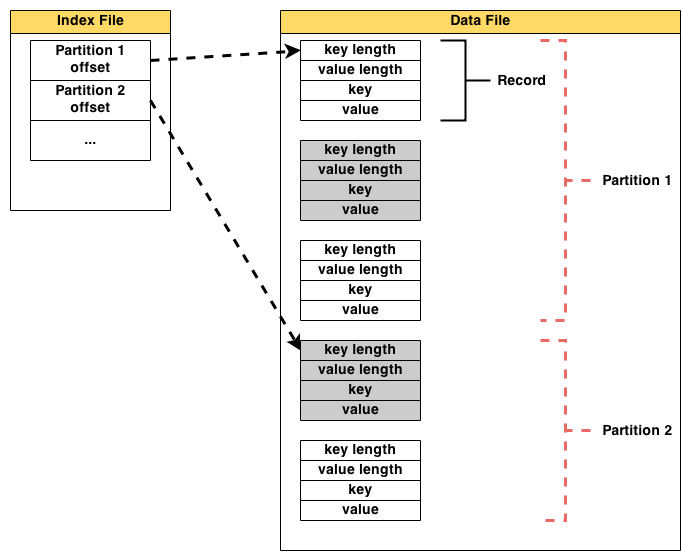
\includegraphics[scale=0.4]{./Figures/spill_partition}
    \end{center}
}

%%%%%%%%%%%%%%%%%%%%%%%%%%%%%%%%%%%%%%%%%%%%%%%%%%%%%%%%%%
\frame {\frametitle{Shuffle and Sort: Reduce Side}
%%%%%%%%%%%%%%%%%%%%%%%%%%%%%%%%%%%%%%%%%%%%%%%%%%%%%%%%%%
   \begin{center}
      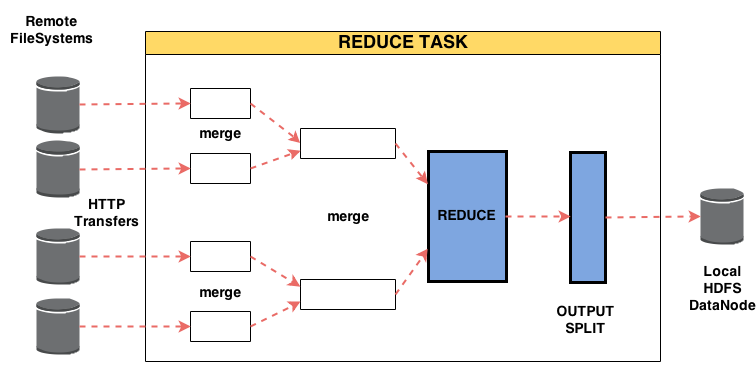
\includegraphics[scale=0.4]{./Figures/reduce_task}
    \end{center}
}

%%%%%%%%%%%%%%%%%%%%%%%%%%%%%%%%%%%%%%%%%%%%%%%%%%%%%%%%%%
\frame {\frametitle{Shuffle and Sort: the Reduce Side}
%%%%%%%%%%%%%%%%%%%%%%%%%%%%%%%%%%%%%%%%%%%%%%%%%%%%%%%%%%
  \begin{itemize}
  \item \textbf{The map output file is located on the local disk of
     TaskTracker}

  \item \textbf{Another TaskTracker (in charge of a reduce task)
      requires input from many other TaskTracker (that finished their
      map tasks)}
    \begin{itemize}
    \item How do reducers know which \texttt{TaskTrackers} to fetch map output
      from?
      \begin{itemize}
      \item When a map task finishes it notifies the parent
        TaskTracker
      \item The TaskTracker notifies (with the heartbeat mechanism)
        the JobTracker
      \item A thread in the reducer {\color{red}polls periodically}
        the \texttt{JobTracker}
      \item \texttt{TaskTrackers} do not delete local map output as soon as a
        reduce task has fetched them ({\color{red}WHY?})
      \end{itemize}
    \end{itemize}

  \item \textbf{Copy phase: a pull approach}
    \begin{itemize}
    \item There is a small number (5) of copy threads that can fetch
      map outputs in parallel
    \end{itemize}
  \end{itemize}
}

%%%%%%%%%%%%%%%%%%%%%%%%%%%%%%%%%%%%%%%%%%%%%%%%%%%%%%%%%%
\frame {\frametitle{Shuffle and Sort: the Reduce Side}
%%%%%%%%%%%%%%%%%%%%%%%%%%%%%%%%%%%%%%%%%%%%%%%%%%%%%%%%%%
  \begin{itemize}
  \item \textbf{The map output are copied to the the TraskTracker running the
      reducer in {\color{red}memory} (if they fit)}
    \begin{itemize}
    \item Otherwise they are copied to disk
    \end{itemize}

    \vspace{20pt}

  \item \textbf{Input consolidation}
    \begin{itemize}
    \item A background thread merges all partial inputs into larger,
      {\color{red}sorted} files
    \item Note that if compression was used (for map outputs to save
      bandwidth), decompression will take place in memory
    \end{itemize}

    \vspace{20pt}

  \item \textbf{Sorting the input}
    \begin{itemize}
    \item When all map outputs have been copied a merge phase starts
    \item All map outputs are sorted maintaining their sort ordering,
      in rounds
    \end{itemize}
  \end{itemize}
}

%%%%%%%%%%%%%%%%%%%%%%%%%%%%%%%%%%%%%%%%%%%%%%%%%%%%%%%%%%
%%%%%%%%%%%%%%%%%%%%%%%%%%%%%%%%%%%%%%%%%%%%%%%%%%%%%%%%%%
\subsection{Types and Formats}
%%%%%%%%%%%%%%%%%%%%%%%%%%%%%%%%%%%%%%%%%%%%%%%%%%%%%%%%%%
%%%%%%%%%%%%%%%%%%%%%%%%%%%%%%%%%%%%%%%%%%%%%%%%%%%%%%%%%%
\begin{frame}
 \begin{colorblock}{blue}{lightblue}{ }
  \begin{center}
    \textbf{Types and Formats}
  \end{center}
  \end{colorblock}
\end{frame}

%%%%%%%%%%%%%%%%%%%%%%%%%%%%%%%%%%%%%%%%%%%%%%%%%%%%%%%%%%
\frame {\frametitle{MapReduce Types}
%%%%%%%%%%%%%%%%%%%%%%%%%%%%%%%%%%%%%%%%%%%%%%%%%%%%%%%%%%
  \begin{itemize}
  \item \textbf{Recall: Input / output to mappers and reducers}
    \begin{itemize}
    \item map: $(k1, v1)$ $\to$ $[(k2, v2)]$
    \item reduce: $(k2, [v2])$ $\to$ $[(k3, v3)]$
    \end{itemize}
    
    \vspace{20pt}

{\color{red}
  \item \textbf{In Hadoop, a mapper is created as follows:}
    \begin{itemize}
    \item \texttt{void map(K1 key, V1 value, Context context)}
    \end{itemize}
}

    \vspace{20pt}

  \item \textbf{Types:}
    \begin{itemize}
    \item $K$ types implement \texttt{WritableComparable}
    \item $V$ types implement \texttt{Writable}
    \end{itemize}
  \end{itemize}   
}

%%%%%%%%%%%%%%%%%%%%%%%%%%%%%%%%%%%%%%%%%%%%%%%%%%%%%%%%%%
\frame {\frametitle{What is a \texttt{Writable}}
%%%%%%%%%%%%%%%%%%%%%%%%%%%%%%%%%%%%%%%%%%%%%%%%%%%%%%%%%%
  \begin{itemize}
  \item \textbf{Hadoop defines its own classes for strings (\texttt{Text}),
    integers (\texttt{intWritable}), etc...}

    \vspace{20pt}

  \item \textbf{All keys are instances of \texttt{WritableComparable}}
    \begin{itemize}
    \item {\color{red}Why comparable?}
    \end{itemize}

    \vspace{20pt}

  \item \textbf{All values are instances of \texttt{Writable}}

  \end{itemize}
}

%%%%%%%%%%%%%%%%%%%%%%%%%%%%%%%%%%%%%%%%%%%%%%%%%%%%%%%%%%
\frame {\frametitle{Getting Data to the Mapper}
%%%%%%%%%%%%%%%%%%%%%%%%%%%%%%%%%%%%%%%%%%%%%%%%%%%%%%%%%%
   \begin{center}
      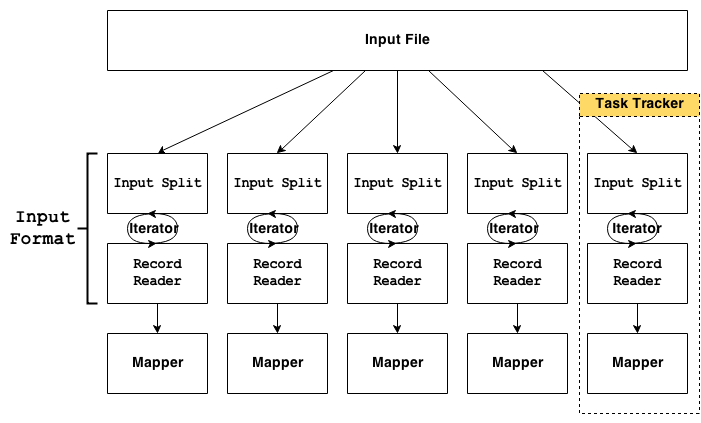
\includegraphics[scale=0.4]{./Figures/data2map}
    \end{center}
}

%%%%%%%%%%%%%%%%%%%%%%%%%%%%%%%%%%%%%%%%%%%%%%%%%%%%%%%%%%
\frame {\frametitle{Reading Data}
%%%%%%%%%%%%%%%%%%%%%%%%%%%%%%%%%%%%%%%%%%%%%%%%%%%%%%%%%%
  \begin{itemize}
  \item \textbf{Datasets are specified by \texttt{InputFormats}}
    \begin{itemize}
    \item \texttt{InputFormats} define input data (e.g. a file, a
      directory)
    \item \texttt{InputFormats} is a factory for \texttt{RecordReader}
      objects to extract key-value records from the input source
    \end{itemize}

    \vspace{20pt}

  \item \textbf{\texttt{InputFormats} identify partitions of the data
      that form an \texttt{InputSplit}}
    \begin{itemize}
    \item \texttt{InputSplit} is a (\textbf{reference to a}) chunk of
      the input processed by a {\color{red}single} map
      \begin{itemize}
      \item Largest split is processed first
      \end{itemize}
    \item Each split is divided into records, and the map processes each
      record (a key-value pair) in turn
    \item Splits and records are {\color{red}logical}, they are not
      physically bound to a file
    \end{itemize}
  \end{itemize}
}

%%%%%%%%%%%%%%%%%%%%%%%%%%%%%%%%%%%%%%%%%%%%%%%%%%%%%%%%%%
\frame {\frametitle{\texttt{InputFormat}}
%%%%%%%%%%%%%%%%%%%%%%%%%%%%%%%%%%%%%%%%%%%%%%%%%%%%%%%%%%
  \begin{itemize}
  \item \textbf{\texttt{TextInputFormat}}
    \begin{itemize}
    \item Treats each \texttt{newline}-terminated line of a file as a value
    \end{itemize}

    \vspace{20pt}

  \item \textbf{\texttt{KeyValueTextInputFormat}}
    \begin{itemize}
    \item Maps \texttt{newline}-terminated text lines of ``key'' SEPARATOR ``value''
    \end{itemize}

    \vspace{20pt}

  \item\textbf{\texttt{SequenceFileInputFormat}}
    \begin{itemize}
    \item Binary file of key-value pairs with some additional metadata
    \end{itemize}

    \vspace{20pt}

  \item \textbf{\texttt{SequenceFileAsTextInputFormat}}
    \begin{itemize}
    \item Same as before but, maps \texttt{(k.toString(), v.toString())}
    \end{itemize}
  \end{itemize}

}

%%%%%%%%%%%%%%%%%%%%%%%%%%%%%%%%%%%%%%%%%%%%%%%%%%%%%%%%%%
\frame {\frametitle{\texttt{InputSplit}}
%%%%%%%%%%%%%%%%%%%%%%%%%%%%%%%%%%%%%%%%%%%%%%%%%%%%%%%%%%
  \begin{itemize}
  \item \textbf{\texttt{FileInputFormat} divides large files into
      chunks}
    \begin{itemize}
    \item Exact size controlled by \texttt{mapred.min.split.size}
    \end{itemize}

    \vspace{20pt}

  \item \textbf{Record readers receive file, offset, and length of chunk}
    \begin{itemize}
    \item Example
    \end{itemize}
    \begin{footnotesize}
      \begin{columns}[c]
        \column{6cm}
        On the top of the Crumpetty Tree$\to$\\
        The Quangle Wangle sat,$\to$\\
        But his face you could not see,$\to$\\
        On account of his Beaver Hat.$\to$\\
        
        \column{6cm}
        
        (0, On the top of the Crumpetty Tree)\\
        (33, The Quangle Wangle sat,)\\
        (57, But his face you could not see,)\\
        (89, On account of his Beaver Hat.)\\
      \end{columns}
    \end{footnotesize}

    \vspace{20pt}

  \item \textbf{Custom \texttt{InputFormat} implementations may
      override split size}
 \end{itemize}
}

%%%%%%%%%%%%%%%%%%%%%%%%%%%%%%%%%%%%%%%%%%%%%%%%%%%%%%%%%%
\frame {\frametitle{The relationship between an \texttt{InputSplit} and an HDFS block}
%%%%%%%%%%%%%%%%%%%%%%%%%%%%%%%%%%%%%%%%%%%%%%%%%%%%%%%%%%
   \begin{center}
      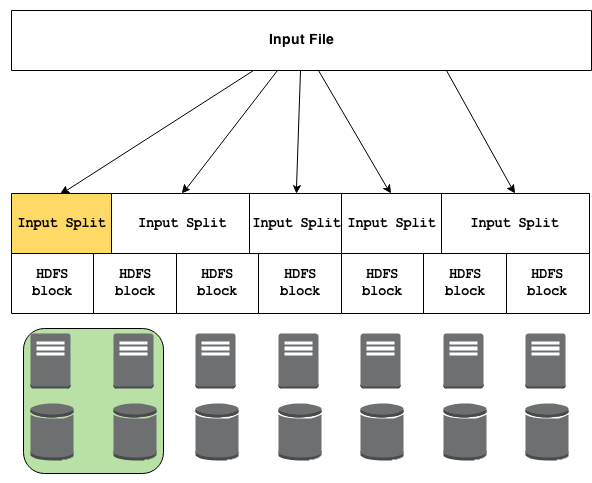
\includegraphics[scale=0.4]{./Figures/split_block}
    \end{center}
}

%%%%%%%%%%%%%%%%%%%%%%%%%%%%%%%%%%%%%%%%%%%%%%%%%%%%%%%%%%
\frame {\frametitle{Record Readers}
%%%%%%%%%%%%%%%%%%%%%%%%%%%%%%%%%%%%%%%%%%%%%%%%%%%%%%%%%%
  \begin{itemize}
  \item \textbf{Each \texttt{InputFormat} provides its own \texttt{RecordReader} implementation}

    \vspace{20pt}
 
  \item \textbf{\texttt{LineRecordReader}}
    \begin{itemize}
    \item Reads a line from a text file
    \end{itemize}

    \vspace{20pt}
 
  \item \textbf{\texttt{KeyValueRecordReader}}
    \begin{itemize}
    \item Used by \texttt{KeyValueTextInputFormat}
    \end{itemize}

  \end{itemize}
}

%%%%%%%%%%%%%%%%%%%%%%%%%%%%%%%%%%%%%%%%%%%%%%%%%%%%%%%%%%
\frame {\frametitle{Sending Data to Reducers}
%%%%%%%%%%%%%%%%%%%%%%%%%%%%%%%%%%%%%%%%%%%%%%%%%%%%%%%%%%
{\color{red}
  \begin{itemize}
  \item \textbf{Map function receives \texttt{Context} object}
    \begin{itemize}
    \item \texttt{Context.write()} receives key-value elements
    \end{itemize}

    \vspace{20pt}
    
  \item \textbf{Any (\texttt{WritableComparable}, \texttt{Writable}) can be
      used}
    
    \vspace{20pt}
    
  \item \textbf{By default, mapper output type assumed to be the same
      as the reducer output type}
    
  \end{itemize}
}
}

%%%%%%%%%%%%%%%%%%%%%%%%%%%%%%%%%%%%%%%%%%%%%%%%%%%%%%%%%%
\frame {\frametitle{WritableComparator}
%%%%%%%%%%%%%%%%%%%%%%%%%%%%%%%%%%%%%%%%%%%%%%%%%%%%%%%%%%
  \begin{itemize}
  \item \textbf{Compares \texttt{WritableComparable} data}
    \begin{itemize}
    \item Will call the \texttt{WritableComparable.compare()} method
    \item Can provide fast path for serialized data
    \end{itemize}

\vspace{40pt}

\item \textbf{Configured through:
    \texttt{JobConf.setOutputValueGroupingComparator()}}
  \end{itemize}
}

%%%%%%%%%%%%%%%%%%%%%%%%%%%%%%%%%%%%%%%%%%%%%%%%%%%%%%%%%%
\frame {\frametitle{Partitioner}
%%%%%%%%%%%%%%%%%%%%%%%%%%%%%%%%%%%%%%%%%%%%%%%%%%%%%%%%%%
  \begin{itemize}
  \item \textbf{\texttt{int getPartition(key, value, numPartitions)}}
    \begin{itemize}
    \item Outputs the partition number for a given key
    \item One partition == all values sent to a single reduce task
    \end{itemize}

    \vspace{20pt}
    
  \item \textbf{\texttt{HashPartitioner} used by default}
    \begin{itemize}
    \item Uses \texttt{key.hashCode()} to return partition number
    \end{itemize}
    
    \vspace{20pt}
    
  \item \textbf{\texttt{JobConf} used to set \texttt{Partitioner} implementation}
  \end{itemize}
  
}

%%%%%%%%%%%%%%%%%%%%%%%%%%%%%%%%%%%%%%%%%%%%%%%%%%%%%%%%%%
\frame {\frametitle{The Reducer}
%%%%%%%%%%%%%%%%%%%%%%%%%%%%%%%%%%%%%%%%%%%%%%%%%%%%%%%%%%
  \begin{itemize}
  {\color{red}\item \textbf{\texttt{void reduce(k2 key, Iterator<v2> values, Context context})}}

    \vspace{20pt}

  \item \textbf{Keys and values sent to one partition all go to the
      same reduce task}

    \vspace{20pt}

  \item \textbf{Calls are sorted by key}
    \begin{itemize}
    \item ``Early'' keys are reduced and output before ``late'' keys
    \end{itemize}
  \end{itemize}
}

%%%%%%%%%%%%%%%%%%%%%%%%%%%%%%%%%%%%%%%%%%%%%%%%%%%%%%%%%%
\frame {\frametitle{Writing the Output}
%%%%%%%%%%%%%%%%%%%%%%%%%%%%%%%%%%%%%%%%%%%%%%%%%%%%%%%%%%
  \begin{itemize}
  \item \textbf{Analogous to \texttt{InputFormat}}

    \vspace{20pt}
    
  \item \textbf{\texttt{TextOutputFormat} writes ``key value <\texttt{newline}>'' strings to output file}

    \vspace{20pt}
    
  \item \textbf{\texttt{SequenceFileOutputFormat} uses a binary format
      to pack key-value pairs}

    \vspace{20pt}

  \item \textbf{\texttt{NullOutputFormat} discards output}
    
  \end{itemize}

}



